\section{Gauss-Laguerre \\ Integration}

The convolution of an exponential decay and a Gaussian resolution function is given by
\begin{equation}
    f(t)=\int^\infty_0 \frac{e^{\frac{-(t-t')^2}{2\sigma^2_t}}}{\sqrt{2\pi\sigma^2_t}}\frac{e^{\frac{-t'}{\tau}}}{\tau}dt'.
    \label{eq:convolution}
\end{equation}

This can be integrated using Gauss-Laguerre Integration. It consists of making the integral into the form:
\begin{equation}
    f(t)=\int^\infty_0 dx w(x) f(x)
\end{equation}
where $w(x)$ is of the form $e^{-x}$. To achieve this form we have to make the following substitution $x=t'/\tau$ and $dx=dt'/\tau$. Then we have the following
\begin{align*}
    f(x)&=\frac{1}{\sqrt{2\pi\sigma_t^2}}\int^\infty_0 e^{-\frac{(t-x\tau)**2}{2\sigma_t^2}}e^{-x} dx\\
    f(x)&=\frac{1}{\sqrt{2\pi\sigma_t^2}}\sum_0^N w(x_i)f(x_i)
\end{align*}
where $x_i$ are the roots of the polynomial of degree $N$ that is being used to approximate the function $f(x)$.

The top plot of Figure \ref{fig:GaussLaguerrePlot} shows the solution of the solution of the integral evaluated at $100$ points for $t\in[-2,6]$, $\tau=1$ and $\sigma_t=0.5$ with values of $N=5,10,15,20,$ and $30$. 

The analytic solution plotted is given by
\begin{equation}
    f(t)=\frac{1}{2\tau}e^{\left(\frac{\sigma^2_t}{2\tau^2}-\frac{t}{\tau}\right)}\mathrm{erfc}\left(\frac{\sigma_t}{\sqrt{2}\tau}-\frac{t}{\sqrt{2}\sigma_t}\right).
    \label{eq:convAnalytic}
\end{equation}

The error can be seen on the middle and bottom plot which correspond to the relative error and the absolute error, respectively. The relative error and absolute error was calculated by 
\begin{align*}
    |(analytic-numeric)/analytic|, \mathrm{and}\\
    |analytic-numeric|,
\end{align*}
respectively. Note that at higher values of $N$ the numeric solution get smaller relative and absolute error.

\begin{figure}
    \centering
    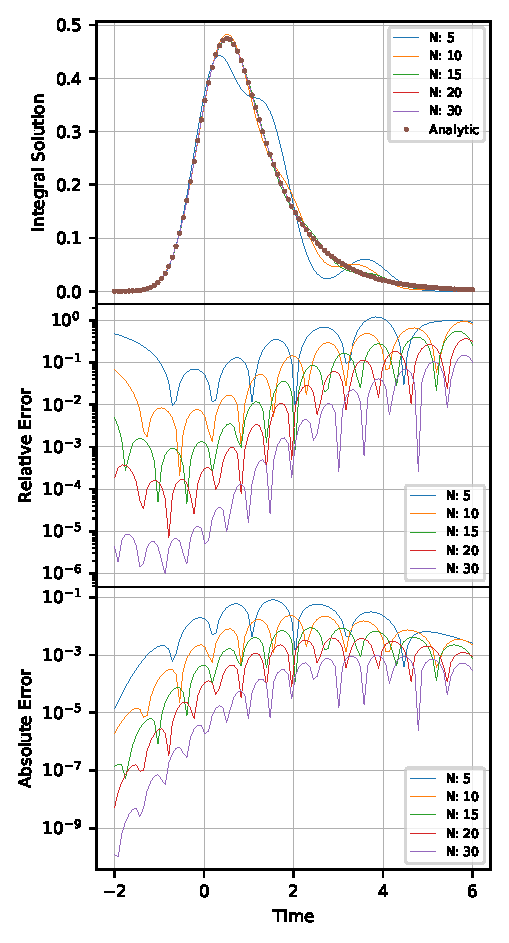
\includegraphics{CodeAndFigures/GaussLaguerreQuadrature.pdf}
    \caption{\emph{Top}: Solution to the integral of equation \ref{eq:convolution} using Gauss-Laguerre quadrature of N degrees for $\tau=1,\sigma_t=0.5$ evaluated at 100 points for $t\in[-2,6]$. \emph{Middle}: Relative error of the analytic solution and numeric solutions. \emph{Bottom}: Absolute error of the analytic solution and numeric solutions.}
    \label{fig:GaussLaguerrePlot}
\end{figure}
